\section{Set-Up}
\begin{figure}[h]
    \centering
    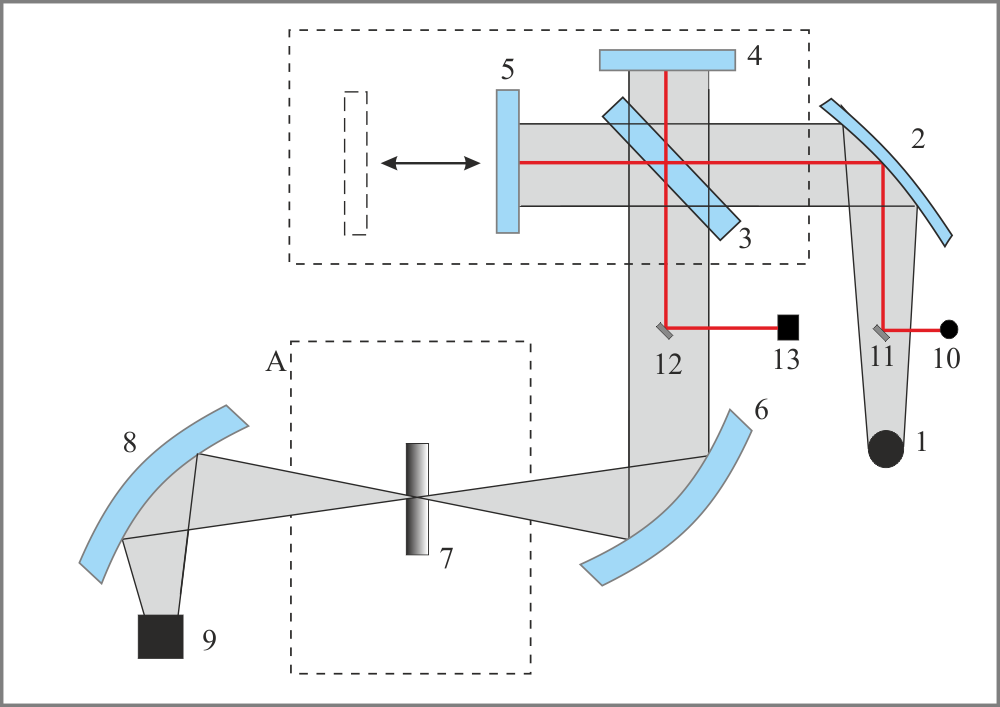
\includegraphics[width=0.4\textwidth]{Images/Aufbau_set_up.png}
    \caption{Simplified schematic illustration of the set-up used for all experiments. A short overview of
    the working principle is given in the text.\cite{Set-Up}}
    \label{fig:set-up}
\end{figure}
Fig.\,\ref{fig:set-up} shows a schematic version of the \emph{Bruker IFS 66 v/s} Fourier spectrometer. 
The source (1) emmits light in the near-
infrared range ($1500\,\text{cm}^{-1} - 15000\,\text{cm}^{-1}$) which is then reflected on the $\text{CaF}_2$ beamsplitter (3) \cite{Anleitung}. 
The beamsplitter, static mirror (4) 
and movable mirror (5) make up a Michelson interferometer which is used to create a interference pattern.
During the measurement, the movable mirror is moved with constant speed.
The light is then focused via another mirror (6) on the sample (7). In fig.\,\ref{fig:set-up} the set-up is used in transmission mode.
For reflection measurements an additional module is used which is not shown in the figure. Mirror (8) then 
focuses the light onto the pyroelectric (DTGS) detector (9). The signal is then digitalized.
Numbers (10) to (13) show the beampath of a laser which is used to determine the position of the movable mirror. 
The system applies a phase 'Mertz' phase correction on the signal and fourier transforms the signal.
The evaluation of the signal with the 'Mertz' phase correction is performed automatically by the system.
